\newpage
$ $
\newpage

\renewcommand{\thesubsection}{\textcolor{red}{\Roman{section}.\arabic{subsection}}}
\renewcommand{\thesubsubsection}{\textcolor{red}{\Roman{section}.\arabic{subsection}.\alph{subsubsection}}}

\setcounter{section}{0}
\sndEnTeteDeux

\begin{center}
\begin{mdframed}[style=titr, leftmargin=60pt, rightmargin=60pt, innertopmargin=7pt, innerbottommargin=7pt, innerrightmargin=8pt, innerleftmargin=8pt]

\begin{center}
\large{\textbf{Chapitre 1 : Corps purs et mélanges au quotidien}}
\end{center}

\end{mdframed}
\end{center}
Ce chapitre permet de faire une description de la matière à l'échelle macroscopique (c'est-à-dire à notre échelle). Posons-nous les questions suivantes. Qu'est-ce qu'une espèce chimique ? Comment faire pour en identifier une en laboratoire ? Comment reconnaître un mélange d'une espèce chimique unique ?
%
\begin{tcolorbox}[colback=blue!5!white,colframe=blue!75!black,title=Mots clés du chapitre :]
Corps purs, mélange homogène/hétérogène, masse volumique, températures de changement d'état, solubilité.
\end{tcolorbox}

%

\section{Définitions}

\subsection{Espèces chimiques}

La matière est constituée d'\textcolor{red}{entités chimiques} : les atomes, les molécules, les ions. \`{A} partir de ces entités, on peut définir une \textcolor{red}{espèce chimique} :
\begin{tcolorbox}[colback=green!5!white,colframe=green!75!black,title=\textbf{Espèce chimique}, upperbox=invisible]
Elle est composée d'un ensemble d'entités chimiques identiques. Une espèce chimique est caractérisée par :
\begin{itemize}
    \item sa formule chimique : par exemple \chemform{H_2O} pour l'eau,
    \item son aspect : couleur, texture, forme, ...
    \item ses propriétés physiques : température d'ébullition, masse volumique, indice de réfraction, ...
    \item ses propriétés chimiques : réactivité avec d'autres espèces chimiques, ... 
    \item 
    \item
\end{itemize}

\end{tcolorbox}

\begin{mdframed}[style=autreexo]
\textbf{\bsc{Exercice de cours 1} - Espèces chimiques}\\
Donner le type (\textit{atomique}, \textit{moléculaire} ou \textit{ionique}) des espèces chimiques suivantes : hélium (He), eau (H\textsubscript{2}O), chlorure de sodium (Na$^{+}$, Cl$^{-}$).
\end{mdframed}

On distingue alors les \textcolor{red}{corps purs} et les \textcolor{red}{mélanges}.

\subsection{Les corps purs}
\begin{tcolorbox}[colback=green!5!white,colframe=green!75!black,title=\textbf{Corps purs}]
Un corps pur est constitué d'une unique espèce chimique.
\end{tcolorbox}

Les corps purs peuvent être :

\begin{itemize}
    \item \textcolor{red}{simples} : ils sont constitués d'un seul type d'atome. Exemples : le dihydrogène \chemform{H_2}, le carbone \chemform{C}, l'argent \chemform{Ag}.
    \item \textcolor{red}{composés} : ils sont constitués de plusieurs atomes dans des proportions bien définies. Exemples : l'eau \chemform{H_2O}, l'éthanol \chemform{C_2H_6O}, le chlorure de sodium \chemform{(Na^+;Cl^-)}.
\end{itemize}

%%%%%%%%



%
\subsection{Le cas des mélanges}
\begin{tcolorbox}[colback=green!5!white,colframe=green!75!black,title=\textbf{Mélange}]
Un mélange est constitué de plusieurs espèces chimiques différentes.
\end{tcolorbox}
Les mélanges peuvent être :
\begin{itemize}
    \item \textcolor{red}{homogènes} : ils sont constitués d'une seule phase (solide, liquide ou vapeur) indiscernable à l'\oe il nu. Lorsque deux liquides se mélangent l'un avec l'autre, on dit qu'ils sont \textcolor{red}{miscibles}.
    \item hétérogènes : 
\end{itemize}
\section{Identification d'espèces chimiques}
Comment reconnaitre une espèce chimique par rapport à une autre ? 

\subsection{Aspects physiques}
Couleur, aspect, goût, état physique à température ambiante.
\subsection{Propriétés physiques}
\subsubsection{La masse volumique}
Def+tableau de quelques masses volumiques connues avec photo.
\subsubsection{Les températures de changement d'état}

\begin{figure}[!htb]
    \centering
    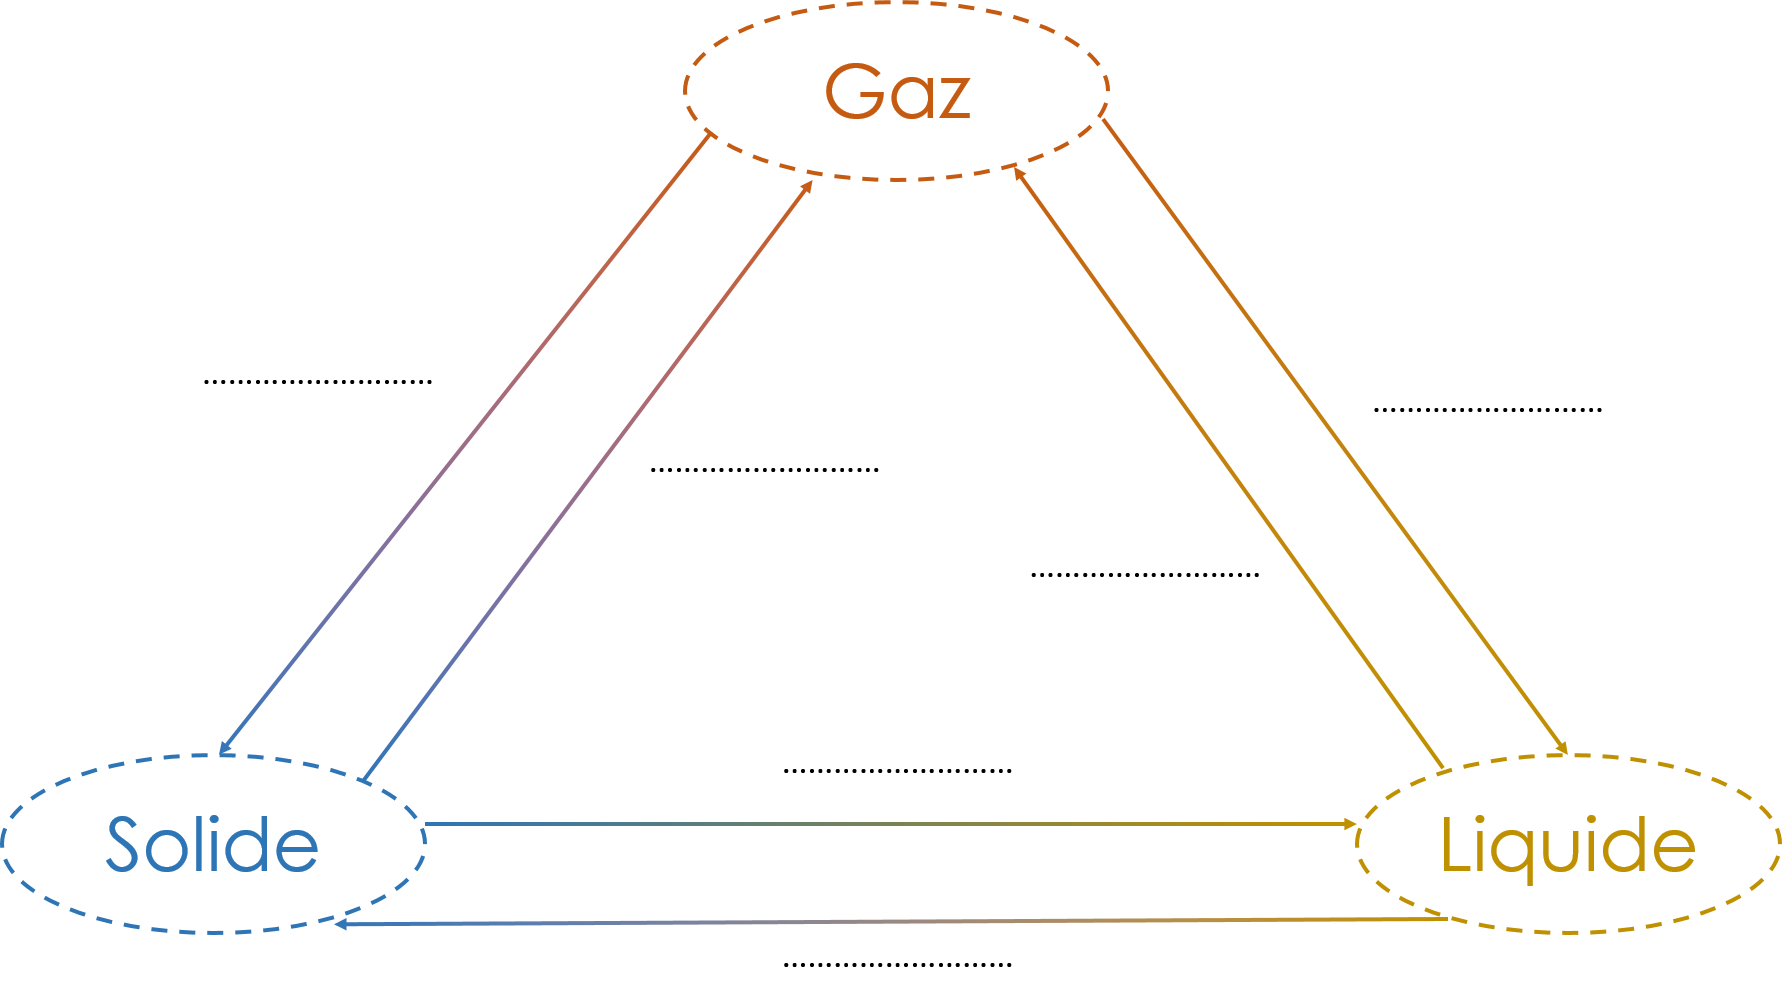
\includegraphics[scale=0.5]{Cours/Changement_etat.png}
    \caption{Les changements d'états de la matière}
    \label{fig:enter-label}
\end{figure}
\subsubsection{La solubilité}
Def + dépendance avec la température.

\section{Composition d'un mélange}
Définition miscibilité, homogènes, hétérogènes. Mettre photo huile+eau, sulfate de cuivre + eau.